\chapter{Evaluierung}
\label{chap:eval}
\todo[size=\small, color=blue!40, inline]{Kapitel: Evaluierung}%
\begin{itemize}
 \item wie skaliert das System / bringt es was?
 \item Balancierung durch $c$-Collision Protokoll / die Varianz
 \item Netzwerk ist wichtig $\rightarrow$ hat sich in den tests gezeigt. Siehe MiniCluster.
\end{itemize}
\todo[size=\small, inline]{Diagramme für Reload: eins mit median und 10\% Quantilen aus einem durchgang; evtl. gemittelt; eins mit min-, oder max-, oder median-werten}%
\todo[size=\small, inline]{absolutes in und max bei den Quantilen angeben und dann einen Block für die Quartile (0.25 und 0.75) und dann den Median eintragen.}%

Um die Effektivität des in dieser Arbeit entstandenen Systems überprüfen zu können, wurden verschiedene Tests durchgeführt.
Beim ersten Test, dem \textit{FPS-Test}, wurden bei einem Walkthrough durch die Szene die Bilder pro Sekunde aufgezeichnet. Der \textit{Reload-Test} hat bei verschiedenen Systemkonfigurationen an festen Kamerapositionen die Zeit gemessen, die ein erneutes Laden der Szene benötigt. Beim \textit{$c$-Collision-Test} wurde die List auf den einzelnen Datenknoten gemessen.\\
Weitere Diagramme und Abbildungen sind in den Anhängen \ref{chap:add_diag} und \ref{chap:add_fig} zu finden.

\section{FPS-Test}
\label{sec:eval:fps}

\todo[inline]{FPS-Test - da muss ich noch mal ran!}
Bei diesem Test wurde in einem festgelegten Walkthrough durch die 3D-Szene gemessen, wieviele Bilder pro Sekunde an welcher Stelle der Szene erreicht werden konnten. Dazu wurden drei verschiedene Konfigurationen getestet:
\begin{itemize}
  \item 2 Renderknoten, je 24, 28 und 32 Datenknoten und Redundanz = 1 
  \item 2 Renderknoten, je 24, 28 und 32 Datenknoten und Redundanz = 2
  \item 2 Renderknoten,je 24, 28 und 32 Datenknoten und Redundanz = 3
\end{itemize}

Redundanz bedeutet, wie oft das Modell der Boeing vollständig im Netzwerk verteilt wurde. An den Diagrammen kann man sehen, dass die FPS im Durchnitt unabhängig von der Anzahl der Datenknoten oder der Redundanzen sind. Dies bedeutet, dass dieses System entkoppelt arbeitet. Es gibt hin und wieder Ausreißer, bei denen die Bildrate über 50 steigt oder bei 1 liegt. Im Grunde die einzelnen Kurven aber recht ähnlich. Die Grafikkarten der Datenknoten sind relativ schwach. Mit eine anderen Cluster-Konfiguration ließen sich möglicherweise andere Ergebnisse feststellen.

\begin{Bild}
%%%%%%%%%%%%%%%%%%%%%%%%%%%%%%%%%%%%%%%%%%%%%%%%%%%%%%%%%
% Beispieldiagramm mit pgfplot und datenfile
%%%%%%%%%%%%%%%%%%%%%%%%%%%%%%%%%%%%%%%%%%%%%%%%%%%%%%%%%

\begin{tikzpicture}
  \begin{axis}[xlabel=Position, ylabel={FPS}]
    \addplot[smooth,red,samples=500] table[col sep=comma,x index=0,y index=1,header=false] {data/FPSWalkthroughTest_Redundance2_R2_D24.2010-1-25.log};
    \addlegendentry{Render2, Data24}
    \addplot[smooth,green,samples=500] table[col sep=comma,x index=0,y index=1,header=false] {data/FPSWalkthroughTest_Redundance2_R2_D28.2010-1-25.log};
    \addlegendentry{Render2, Data28}
    \addplot[smooth,blue,samples=500] table[col sep=comma,x index=0,y index=1,header=false] {data/FPSWalkthroughTest_Redundance2_R2_D32.2010-1-25.log};
    \addlegendentry{Render2, Data32}
  \end{axis}
\end{tikzpicture}

  \captionof{figure}{\label{fig:eval:fps2}FPS in einem Walkthrough. (Redundanz$=$2, 2 Renderer und 24-32 Datenknoten)}
\end{Bild}

\section{Reload-Test}
\label{sec:eval:reload}

Beim Reload-Test wurde gemessen, wie lange die einzelnen Datenknoten benötigen, bei festgelegten Kamerapositionen die Szene komplett zu laden. Dazu wurden sämtliche auf den Renderern befindliche Objekte verworfen und erneut angefordert. Wenn ein Datenknoten mit der kompletten Arbeit fertig war, hat er sich beim Masterknoten gemeldet.\\
Die Diagramme enthalten auf der x-Achse die Kameraposition und auf der y-Achse die normalisierte Zeit. Davon ausgehend, dass bei einem Testlauf nur ein einzige Datenknoten Aufträge bekäme, wäre seine zeitliche laste bei 1.0. In den Diagrammen ist zu erkennen, dass der Median bei allen Diagrammen sehr nah am Durchschnitt liegt. Das bedeutet, dass das System sehr gut balanciert. Alle Datenknoten benötigen für einen Testlauf eine ähnliche Zeit. Es gibt auch hier ab und zu Ausreißer. An den Quartilen lässt sich jedoch erkennen, dass 50\% der Datenknoten näher am Median liegen, als an den Extrema.\\
Die Zeit, die benötigt wird um die gesamte Szene zu laden ist gleich dem Maximum der gemessenen Zeiten der Datenknoten. Dieses Maximum variiert zwar stark, allerdings ist zu bedenknen, dass es sich bei den gemessenen Zeit um Sekunden handelte. Diese unterscheiden sich, je nach Kameraposition, nur im Hundertstel oder Tausendstel-Bereich.\\
Was jedoch auffällt: 24 Datenknoten unterscheiden sich zu 32 Datenknoten darin, dass die einzelnen Knoten weniger Zeit für ihre Aufträge benötigen und somit die Szene auch schneller geladen ist.

\begin{Bild}
%%%%%%%%%%%%%%%%%%%%%%%%%%%%%%%%%%%%%%%%%%%%%%%%%%%%%%%%%
% Beispieldiagramm mit pgfplot und datenfile
%%%%%%%%%%%%%%%%%%%%%%%%%%%%%%%%%%%%%%%%%%%%%%%%%%%%%%%%%

\begin{tikzpicture}
  \begin{axis}[xlabel=Kameraposition, 
	       ylabel={Zeit (normalisiert)},xtick=\empty]
  \addplot[color=red,
	   mark=|,dashed,
	   only marks,
	   error bars/.cd,
	   y dir=both,
	   y explicit,
	   error bar style={red, error bars options={line width=2pt}}]
    table[col sep=comma,x index=0,y index=2,y error index=3, header=false]
    {data/ReloadTest_Redundance2_R2_D32.2010-1-27.log_medians.data};
  \addlegendentry{Extrema}
  \addplot[color=cyan,
	   mark=|,
	   only marks,
	   error bars/.cd,
	   y dir=both,
	   y explicit,
	   error bar style={cyan, very thick},
	   ultra thick] 
    table[col sep=comma,x index=0,y index=4,y error index=5, header=false]
    {data/ReloadTest_Redundance2_R2_D32.2010-1-27.log_medians.data};
  \addlegendentry{Quartile}
  \addplot[color=black,
	   mark=x,
	   only marks] 
    table[col sep=comma,x index=0,y index=1, header=false]
    {data/ReloadTest_Redundance2_R2_D32.2010-1-27.log_medians.data};
  \addlegendentry{Median}
  \addplot[color=green,
	   no marks] 
    table[col sep=comma,x index=0,y index=6, header=false]
    {data/ReloadTest_Redundance2_R2_D32.2010-1-27.log_medians.data};
  \addlegendentry{Average}
  \end{axis}
\end{tikzpicture}
  \captionof{figure}{Reloadtest: Redundanz 2, 2 Renderknoten, 32 Datenknoten.}
\end{Bild}

\begin{Bild}
%%%%%%%%%%%%%%%%%%%%%%%%%%%%%%%%%%%%%%%%%%%%%%%%%%%%%%%%%
% Beispieldiagramm mit pgfplot und datenfile
%%%%%%%%%%%%%%%%%%%%%%%%%%%%%%%%%%%%%%%%%%%%%%%%%%%%%%%%%

\begin{tikzpicture}
  \begin{axis}[xlabel=Kameraposition, 
	       ylabel={Zeit (normalisiert)},xtick=\empty]
  \addplot[color=red,
	   mark=|,dashed,
	   only marks,
	   error bars/.cd,
	   y dir=both,
	   y explicit,
	   error bar style={red, error bars options={line width=2pt}}]
    table[col sep=comma,x index=0,y index=2,y error index=3, header=false]
    {data/ReloadTest_Redundance2_R2_D24.2010-1-27.log_medians.data};
  \addlegendentry{Extrema}
  \addplot[color=cyan,
	   mark=|,
	   only marks,
	   error bars/.cd,
	   y dir=both,
	   y explicit,
	   error bar style={cyan, very thick},
	   ultra thick] 
    table[col sep=comma,x index=0,y index=4,y error index=5, header=false]
    {data/ReloadTest_Redundance2_R2_D24.2010-1-27.log_medians.data};
  \addlegendentry{Quartile}
  \addplot[color=black,
	   mark=x,
	   only marks] 
    table[col sep=comma,x index=0,y index=1, header=false]
    {data/ReloadTest_Redundance2_R2_D24.2010-1-27.log_medians.data};
  \addlegendentry{Median}
  \addplot[color=green,
	   no marks] 
    table[col sep=comma,x index=0,y index=6, header=false]
    {data/ReloadTest_Redundance2_R2_D24.2010-1-27.log_medians.data};
  \addlegendentry{Average}
  \end{axis}
\end{tikzpicture}
  \captionof{figure}{Reloadtest: Redundanz 2, 2 Renderknoten, 24 Datenknoten.}
\end{Bild}

\section{\textit{c}-Collision-Test}
\label{sec:eval:ccollision}

Der Test für das $c$-Collision Protkoll wurde als Einziger nicht im Cluster durchgeführt, sondern ausschließlich in einer Simulation. Dafür wurden alle Anfragen bei einem Walkthrough durch den Cluster aufgezeichnet, unmittelbar bevor sie durch das $c$-Collision Protkoll vergeben wurden. Anschließend wurden diese Aufzeichnungen genutzt, um eine beliebige Datenknotenmenge zu simulieren. Dieser Test arbeitet mit 24, 80 und 120 Datenknoten. Dabei wurde die Last in Form von Dreiecken gemessen, die in jedem Frame an jeden Datenknoten vergeben wurde.\\
Das linke Diagramm zeigt jeweils die Walkthrough-Position (x-Achse) in Relation zur Lastverteilung (y-Achse). Das rechte Diagramm zeigt jeweils die Anfragenmenge, die durch das $c$-Collisione protkoll verteilt wurden (x-Achse) in Relation zur Lastverteilung (y-Achse). Bei Betrachtung des linken Diagramms fallen einige Positionen auf, an denen die Last sehr ungleich verteilt ist und der Median 0 ist. Im rechten Diagramm kann man sehen, dass dies immer dann der Fall ist, wenn sehr wenige Anfragen an das $c$-Collision Protkoll übergeben wurden. Dieses Protokoll dient dazu, Bälle in Körbe zu verteilen. Hat viel weniger Bälle als Körbe, ist das System natürlich nicht gleichmäßig balanciert. Diese Aufträge werden nicht weiter unterteilt. Je nach Zufallsverteilung der Daten auf den Knoten, kann es bei zu geringen Redundanzen auch vorkommen, dass die Wenigen Aufträge nur auf wenige Knoten verteilt werden können.

\begin{itemize}
\item $c$-Collision: Mehr Redundanz = Mittlere Auslastung wird reduziert (blaue durchscnittsdistanz zum median)
\item $c$-Collision: Last ist gut verteilt, wenn Anzahl an Requests hinreichend groß ist
\item $c$-Collision: Bei wenigen Anfragen sehr unbalanciert = wenige Knoten haben überhaupt was zu tun
\item $c$-Collision: Wenige Anfragen = wenig zu sehen (3. drittel, gang aus dem Flugzeug raus = keine Objekte)
\item $c$-Collision: Mehr Knoten = mehr Ausgeglichenheit bei Imbalance-Peaks $\rightarrow$ kann aber sein, dass das einfach durch die Knotenmenge runterskaliert wird. Die Anfragenzahl ist ja gleich.
\end{itemize}

\begin{Bild}
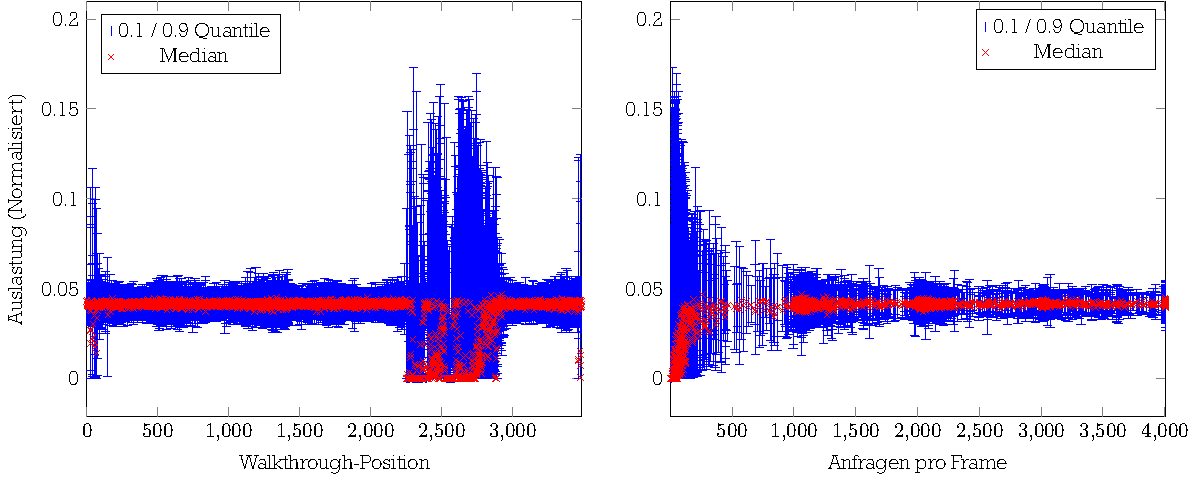
\includegraphics[scale=0.75]{images/diag_cCol_red1_render4_data24_2x.pdf}
  \captionof{figure}{\label{fig:eval:cCol1}Die Auslastung der Datenknoten in einem Walkthrough bei 4 Renderknoten und 24 Datenknoten und Redundanz$=$1.}
\end{Bild}

\begin{Bild}
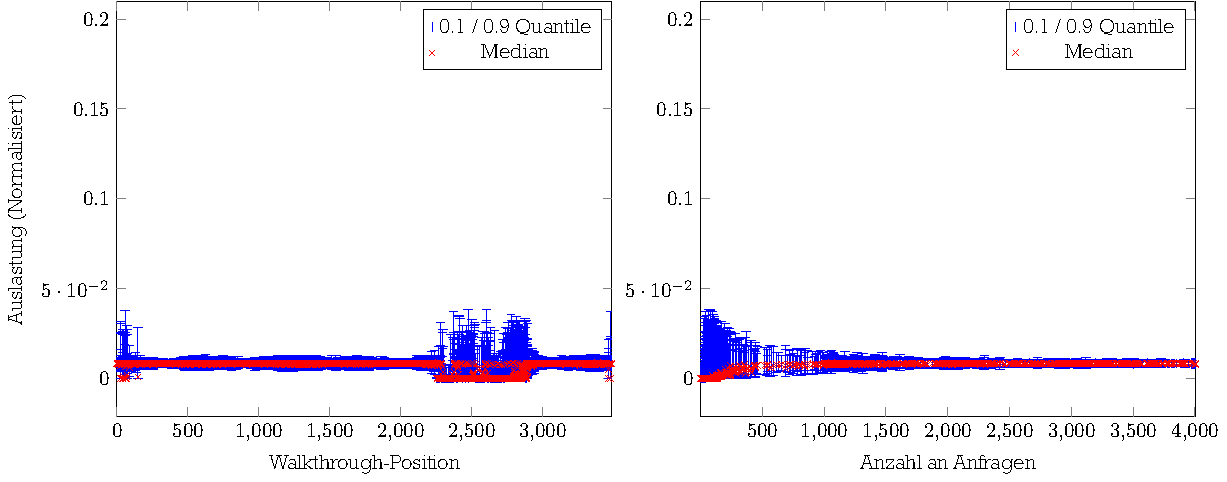
\includegraphics[scale=0.75]{images/diag_cCol_red3_render4_data120_2x.pdf}
  \captionof{figure}{\label{fig:eval:cCol9}Die Auslastung der Datenknoten in einem Walkthrough bei 4 Renderknoten und 120 Datenknoten und Redundanz$=$3.}
\end{Bild}
